\section{Ein Heap Overflow}
\subsection{a) Beschreiben Sie kurz den Sinn und Zweck dieses Programms.}
Das Notetaker-Programm funktioniert, wie der Name schon verrät, als Programm, um sich Notizen abzuspeichern. Dabei wird die Notiz oder Nachricht, die man sich abspeichern will, als Übergabeparameter angenommen und in einen festgeschriebenen Pfad für Notizen abgespeichert.
\subsection{ b) In Ihrer Umgebung finden Sie das Buch hacking art of exploitation 2nd edition.
	Setzen Sie den in Abschnitt 0x341 beschriebenen Angriff auf Ihrem System um. Beschreiben
	Sie dabei die wesentlichen Schritte dieses Angriffs. Begründen Sie, warum dieser Angriff praxisrelevant ist.}
Bei diesem Angriff erzeugen wir durch das Notetaker-Programm einen Heap Overflow, mit dem wir uns dann folgend Root-Zugriff beschaffen können.\\
Als Basis hierfür hatten wir den Abschnitt zum Heap Overflow aus dem Buch Hacking: The Art of Exploitation.\\
Beim Heap reservieren Programmierer fest Speicherplatz und müssen diesen auch wieder freigeben. Dabei wird eine feste Größe angegeben. Ebenso auch beim Notetaker, bei dem wir Speicher reservieren für die zu speichernden Notizen und für den Pfad. 
Unser erstes Argument, also das, was wir als Notiz speichern wollen, wird mit strcpy in einen Buffer geschrieben, und da kann wieder ein Overflow passieren, den wir im Folgenden ausnutzen und damit den Pfad, der ebenfalls auf dem Heap liegt, überschreiben können.\\
Wir bekommen den Speicherbereich durch einfache Ausführung des Programms angezeigt und können somit berechnen, wie groß unser Input sein muss, damit wir einen Overflow erzeugen und den Pfad ändern, in den wir hineinschreiben.
Dafür berechnen wir die Größe wie folgt:
\begin{figure}[H]
	\raggedright
	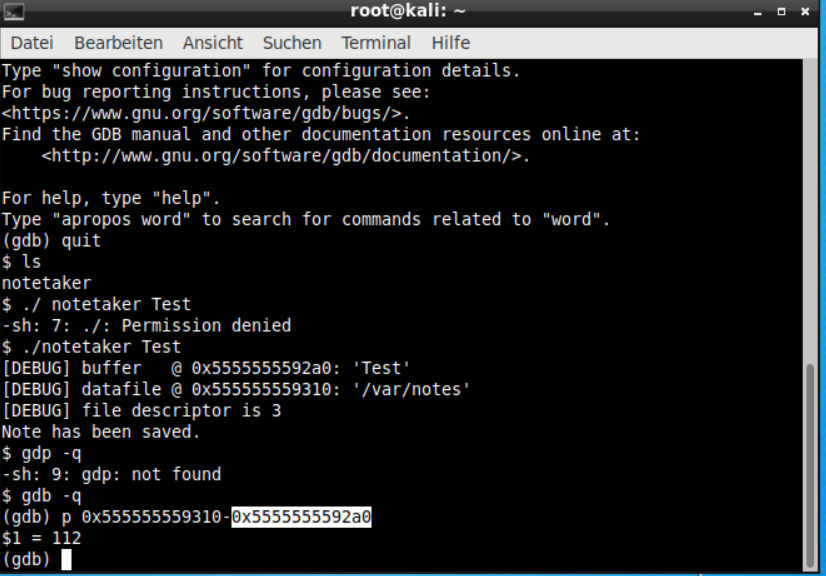
\includegraphics[width=0.7\textwidth]{Bilder/Speicherdifferenz.png}
	\caption{Offset Bestimmen}
	\label{fig:Speicherdifferenz}
\end{figure}
Dafür bilden wir dann unseren String, sodass wir genau diesen Offset treffen und anschließend den Pfad überschreiben können. Wir wollen einen neuen Nutzer in der /etc/passwd anlegen, dabei hat der Input folgende Struktur:
\begin{verbatim}
	benutzername:passwort:UID:GID:GECOS:home-verzeichnis:shell
\end{verbatim}
Daraus ergibt sich für uns folgende Zeile, die wir anfügen wollen:
\begin{verbatim}
	myroot:XXq2KiyI43A2:0:0: <Platz für overflow>:/root:/bin/bash
\end{verbatim}
Da wir aber trotz Overflow die vollständige Zeile des ersten Buffers schreiben müssen, müssen wir für die Shell noch einen kleinen Trick anwenden, indem wir /tmp/etc/passwd auf /bin/bash referenzieren lassen:
\begin{verbatim}
	$   mkdir	tmpetc
	$	ln	-s	binbash	tmpetc/passwd
	$	ls	-l	tmpetc/passwd -> wenn alles richtig wird hier die Referenzierung angezeigt als output der Zeile
\end{verbatim}
Bevor wir den Nutzer hinzufügen, bestimmen wir nun noch die Anzahl an 'A's, die wir schreiben müssen, um den Speicherbereich vollständig zu befüllen.
\begin{figure}[H]
	\raggedright
	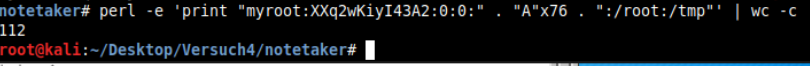
\includegraphics[width=0.7\textwidth]{Bilder/Kali_abstandbufferpasst.png}
	\caption{Overflow String}
	\label{fig:Buffer}
\end{figure}
Nun fügen wir also unseren Nutzer der /etc/passwd hinzu.
\begin{figure}[H]
	\raggedright
	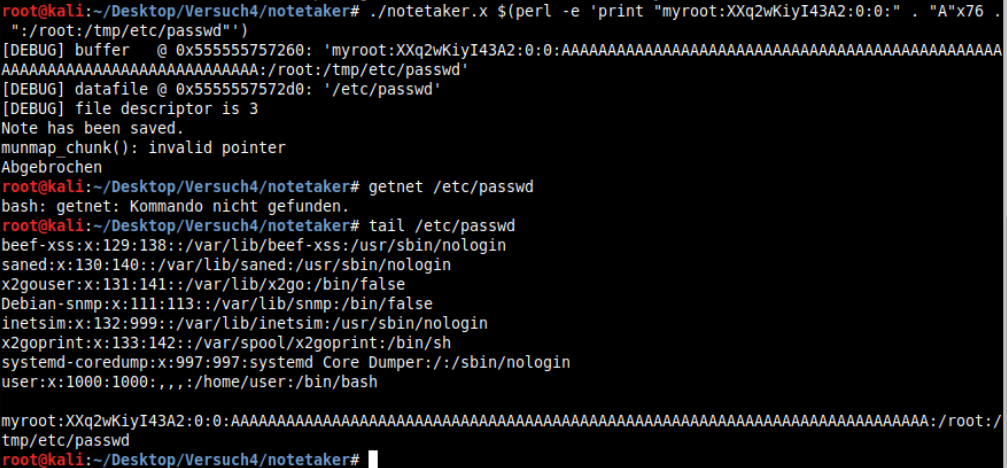
\includegraphics[width=0.7\textwidth]{Bilder/passwd_modifiziert_kali.png}
	\caption{Nutzer angelegt}
	\label{fig:Nutzerangelegt}
\end{figure}
Damit haben wir einen weiteren Root-Nutzer.\\
Dieser Angriff ist praxisrelevant, da es immer die Frage ist, wie es weitergeht, sobald ich Zugriff zu einem System habe. Da ich häufig nicht direkt Root-Rechte habe, sind Programme, die aber Schreib- oder Leserechte im Root-Sinne haben, immer hilfreiche Tools, um weiter in das System hineinzukommen.

\subsection{Führen Sie danach den Angriff gegen das Zielsystem 192.168.1.72 durch. Der Zugriff auf das System selbst erfolgt wieder über SSH und den aus Übung 3 bekannten Nutzernamen sowie dessen Passwort. Hierdurch erhalten Sie im Erfolgsfall und damit verbunden Superuser-Rechten wieder Zugang zu dem Token des in EDX geforderten Users.}
Auch hier beginnen wir nach dem gleichen Prinzip und fügen über das Notetaker-Programm einen neuen Nutzer auf unserem Target-System hinzu.\\
\begin{figure}[H]
	\raggedright
	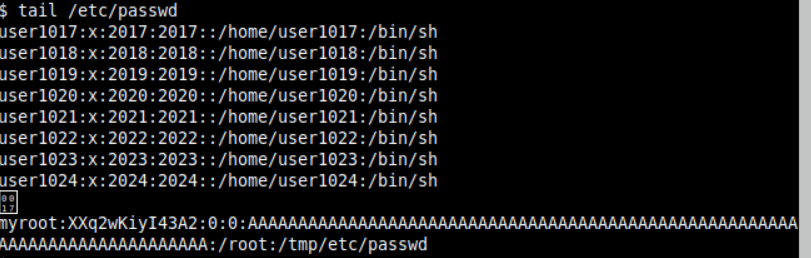
\includegraphics[width=0.7\textwidth]{Bilder/Userangelegt.png}
	\caption{Nutzer angelegt}
	\label{fig:Nutzerangelegt}
\end{figure}
Hier funktioniert su nicht direkt, da wohl weitere Vorkehrungen getroffen wurden, sodass in diesem System nicht jeder Nutzer einfach zu einem Root-Nutzer switchen kann.\\
Daher schauen wir uns die Bedingungen folgend einmal an, indem wir die /etc/pam.d/su-Datei anschauen.
\begin{figure}[H]
	\raggedright
	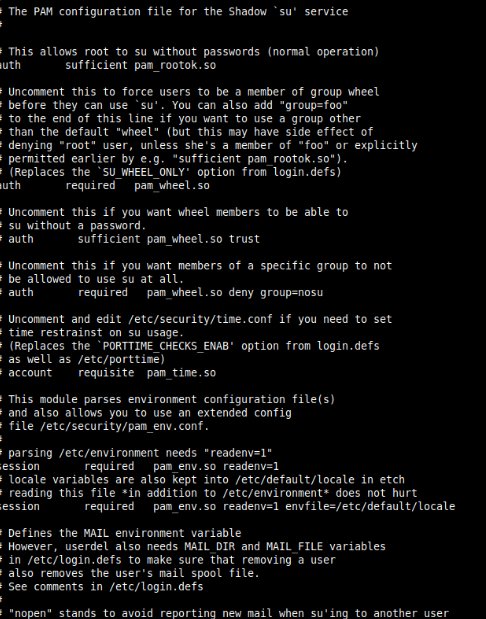
\includegraphics[width=0.7\textwidth]{Bilder/Pam.png}
	\caption{Nutzer angelegt}
	\label{fig:pam-su}
\end{figure}
Hier können wir erkennen, dass einkommentiert ist, dass ein Nutzer der wheel-Gruppe angehörig sein muss.\\
In die Liste der Gruppen geschaut, welche es auf dem System gibt, ist wheel noch nicht hinzugefügt, was uns in die Karten spielt, da wir dadurch einfach eine weitere Zeile an die /etc/groups-Datei anhängen können und die wheel-Gruppe erstellen.\\
Dafür haben wir Folgendes unserem Notetaker-Programm übergeben: 
\begin{figure}[H]
	\raggedright
	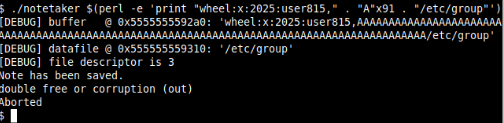
\includegraphics[width=0.7\textwidth]{Bilder/gruppe hinzugefügt.png}
	\caption{Nutzer angelegt}
	\label{fig:gruppehinzu}
\end{figure}
Das hat dazu geführt, dass unser User einer weiteren Gruppe zugehörig ist, was wir mit ID prüfen können.\\
\begin{figure}[H]
	\raggedright
	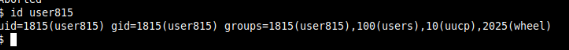
\includegraphics[width=0.7\textwidth]{Bilder/id user.png}
	\caption{user815 Gruppen}
	\label{fig:user}
\end{figure}
Damit hatten wir dann die nötigen berechtigungen um zu unserem neuen Root user zu su und uns damit selber Root rechte verschafft haben.\\
\begin{figure}[H]
	\raggedright
	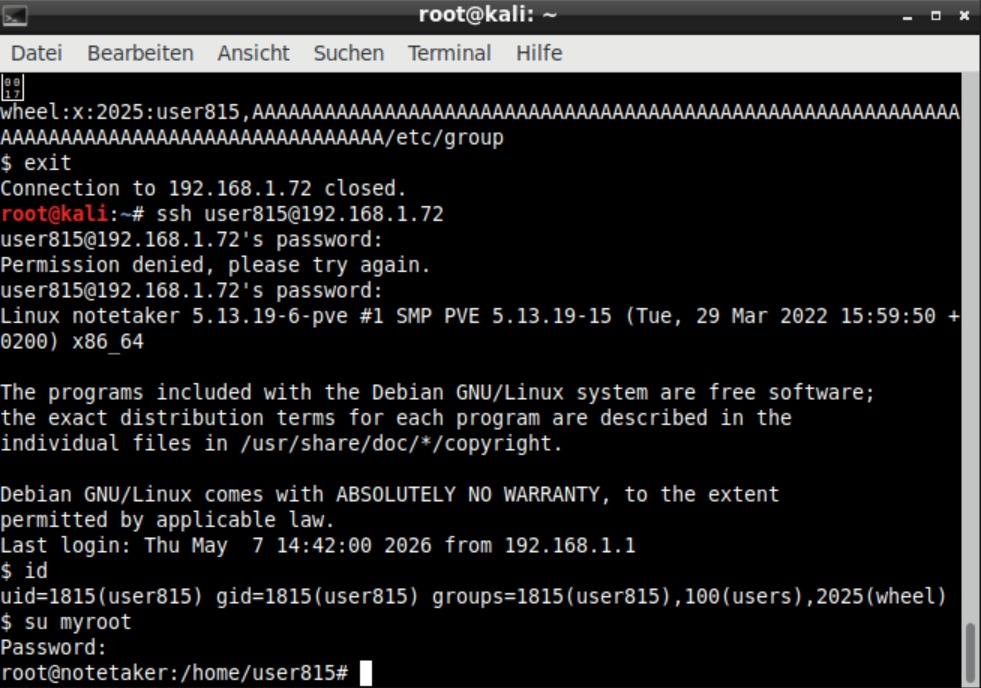
\includegraphics[width=0.7\textwidth]{Bilder/root_notetaker.jpeg}
	\caption{Root Benutzer}
	\label{fig:root}
\end{figure}